\documentclass{article}
\usepackage[utf8]{inputenc}
\usepackage{longtable}
\usepackage{gensymb}
\usepackage{graphicx}
\usepackage{siunitx}
\usepackage{caption}
\usepackage[colorlinks,bookmarks=false,citecolor=blue,linkcolor=blue,urlcolor=blue]{hyperref}
\usepackage{relsize}
\usepackage{amsmath}
\usepackage{booktabs}
\usepackage{amssymb}
\usepackage{bm}
\usepackage{multirow}
\usepackage{placeins}
\begin{document}
\begin{titlepage}
\begin{center}

\includegraphics[scale=0.12]{document/niser.png}
\line(1,0){345}\\
[1mm]
\begin{large}
\textbf{\LARGE Polarization of Light using Wave Plates and Study of Birefringence }\\ 
\end{large}
\line(1,0){240}\\
[5cm]
\large MAITREY SHARMA\\
\small (1911093)\\
[3.5cm]
Third Year Integrated M.Sc.\\
\textbf{School of Physical Sciences}\\
\textbf{National Institute of Science Education and Research, Bhubaneshwar}\\
\small November 16, 2021
\end{center} 
\end{titlepage}
\newpage
\section{Aim}
\begin{itemize}
    \item Measuring the light intensity as function of the analyzer position.
    \item Using the quarter wave plate to produce circularly polarized light.
    \item To study the effect of polarization of a plane polarized light by half wave plate and quarter wave plate.
    \item To measure the intensity at different angles and verify the phenomenon of linear and circular polarization.
\end{itemize}

\section{Apparatus}
\begin{itemize}
    \item Light source,
    \item Polarizer,
    \item Analyzer,
    \item Half-wave plate,
    \item Full-wave plate,
    \item Photo detector.
\end{itemize}

\section{Introduction}
\noindent
A wave plate or retarder is an optical device that alters the
polarization state of a light beam travelling through it. A typical wave plate is simply a birefringent crystal or a double
refracting plastic foil with a carefully chosen thickness. 
\par
\noindent
If a beam of parallel light strikes perpendicularly a wave plate
the light beam is splitted into two components due to its double refracting properties. The two components have planes of
oscillation perpendicular to each other and slightly different
phase velocities. For a quarter-wave plate the thickness of
the foil is chosen in such a manner that the light component
whose electric field vector oscillates in parallel to the rotation
lever lags by a $\lambda /4$ behind other perpendicular oscillating light
component. For a half-wave plate the thickness is chosen so
that the created phase difference has the amount of $\lambda /2$.
\par
\noindent
In this experiment monochromatic light falls on a quarter-wave and half-wave plate. The polarization of the emergent
light is investigated at different angles between the optic axis
of the wave plates and the direction of the incident light. 
\begin{figure}
    \centering
    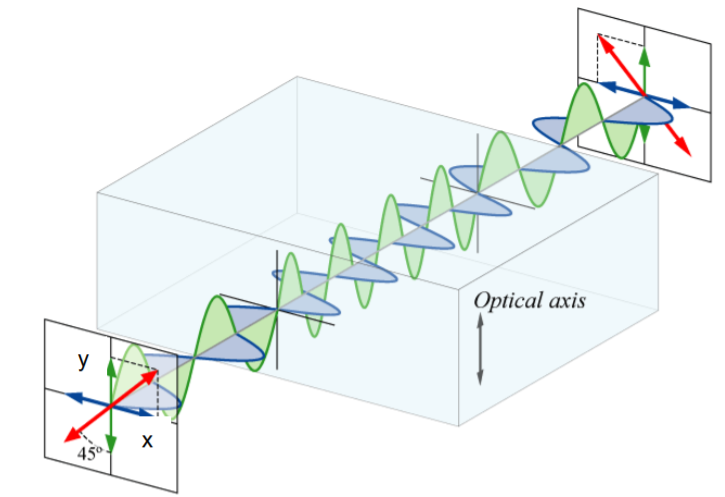
\includegraphics[scale = 0.79]{Figures/halfwaveplate.png}
    \caption{A half-wave plate schematically. Linearly polarized light entering a wave plate can be resolved into two waves, parallel (shown as green) and perpendicular (blue) to the optical axis of the wave plate. In the plate the parallel wave propagates slightly slower than the perpendicular one. At the far side of the plate the parallel wave is exactly half of a wavelength delayed relative to the perpendicular wave. }
    \label{fig:halfwaveplate}
\end{figure}


\section{Schematic}

\begin{figure}[!htb]
    \centering
    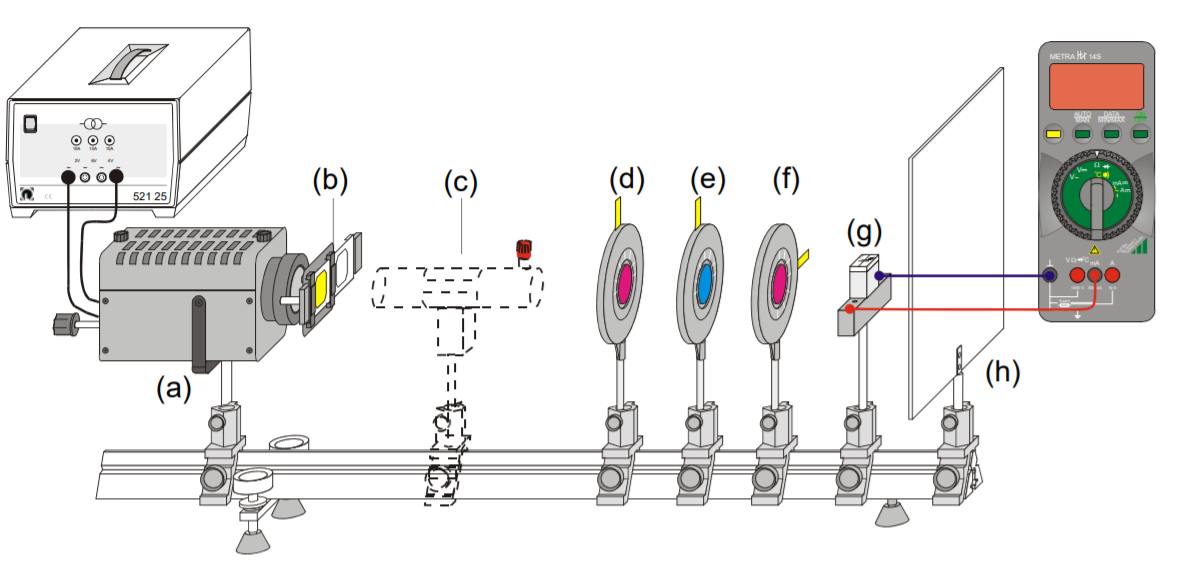
\includegraphics[scale = 0.45]{Figures/schematic.png}
    \captionsetup{justification=centering}
    \caption{Experimental setup for investigating the type of polarization of the emergent light (schematically). (a) halogen lamp (d) polarizer (g) Si photo cell (b) picture slider with filters (e) $\lambda /4$ or $\lambda /2$ wave plate (h) translucent screen (c) heat protection filter (f) analyzer}
    \label{fig:schematic}
\end{figure}



\section{Theory}
\noindent 
A retarder (or waveplate) resolves a light wave into two orthogonal linear polarization components by producing a phase shift between them. The type of polarization depends on this phase difference. 
\par
A retarder is an anisotropic slab that has different magnitudes of refractive indices along its different axes. Light waves can be thought of as the superposition of two perpendicular components once it enters the retarder. Thus, the components experience different refractive indices. The speed of light in a medium is inversely proportional to its refractive index. Hence, one component lags the other in phase.
\par
The two types of retarders we consider are: \textbf{Half-Wave and Quarter-Wave Plates}. A half wave plate retards one component by $180^{\circ}$. In terms of the path difference, there is a shift by $\tfrac{\lambda}{2}$ i.e. half a wave.
A quarter wave plate retards one component by $90^{\circ}$ i.e. by $\tfrac{\lambda}{4}$ or quarter of a wave.
$E_0$ is the amplitude of the electric field vector emerging from 
the polarizer and $\varphi$ the angle between the polarizer and the 
quarter wave plate. At a time $t$ the state of vibration of the two 
component rays is described by:
\begin{equation}
    \begin{split}
        E_1 (t) 
        &= E_0 (t) \cdot \sin \varphi t \cdot \sin \omega \cdot t \\
        E_2 (t)
        &= E_0 (t) \cdot \cos \varphi t \cdot \sin \omega \cdot t
    \end{split}
\end{equation}
\par
\noindent
In the case of the double refracting quarter wave plates the 
thickness causes a path difference of $\lambda /4$ (i.e. a phase difference of $\pi /2$) between the two rays. When emerging the quarter wave plate they combine to a resultant ray which can be 
described by the parametric equations:
\begin{equation}
    \begin{split}
        E_1 (t) 
        &= E_0 \cdot \sin \varphi t \cdot \sin \omega \cdot t \\
        E_2 (t)
        &= E_0 \cdot \cos \varphi t \cdot \sin \omega \cdot t
    \end{split}
\end{equation}
These equation describe an rotating E vector in the direction 
of propagation, i.e. perpendicular to the x- and y-axis about a 
fixed axis (\ref{fig:halfwaveplate}). For the angles $\varphi = \SI{0}{\degree}$ and $\varphi = \SI{90}{\degree}$ we obtain plane polarized 
light intensity after the quarter wave plate:
\begin{equation}
    I = I_0 \sim E_0^2
\end{equation}
For an angle $\varphi = \SI{45}{\degree}$, $\sin \varphi = \cos \varphi = \dfrac{1}{\sqrt{2}}$ and the amount of  the rotating E vector is given by:
\begin{equation}
    E = \sqrt{E_1^2 + E_2^2} = \dfrac{E_0}{\sqrt{2}}
\end{equation}
The light is circularly polarized and the intensity is given by:
\begin{equation}
    I = \dfrac{I_0}{2} \sim \dfrac{E_0^2}{2}
\end{equation}
At all other angles $\varphi$ other that $0 \degree, 45 \degree, 90 \degree$ the transmitted 
light is elliptically polarized. The tip of the $E$ vector rotating 
about the axis parallel to the direction of propagation describes an ellipse with the semi axes $a$ and $b$:
\begin{equation}
    \begin{split}
        E_a (t) 
        &= E_0 \cdot \sin \varphi t \cdot \sin \omega \cdot t \\
        E_b (t)
        &= E_0 \cdot \cos \varphi t \cdot \sin \omega \cdot t
    \end{split}
\end{equation}
The intensity for any angle $\varphi$ between analyzer and quarter 
wave plate (here e.g. $\varphi = \SI{30}{\degree} = \SI{60}{\degree}$) is given by: 
\begin{equation}
    I \sim E_0^2 \cos^2 \varphi \cos^2 \alpha + E_0^2 \sin^2 \varphi \sin^2 \alpha
\end{equation}
The half wave plate produces plane polarized light. For different positions $\varphi$ of the half wave plate only the polarization 
plane changes. For example, if the position of the half wave 
plate is changed about $45 \degree$ the polarization plane changes 
about $90 \degree$. 
\begin{figure}
    \centering
    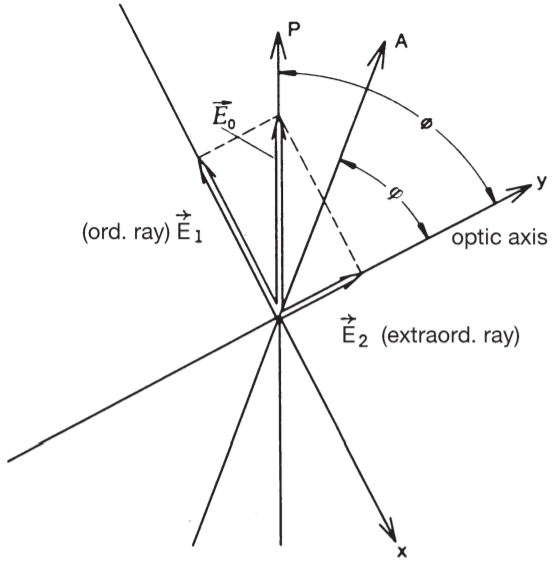
\includegraphics[scale = 0.5]{Figures/splitpolar.png}
    \caption{Splitting of polarised light in a double-refracting crystal (P = polarizer, A = analyzer).}
    \label{fig:my_label}
\end{figure}
\textbf{Linear polarization} is when the different components of the light wave a retarded such that there is a phase difference of $0^\circ$, $180^\circ$ or $360^\circ$ between them. \textbf{Elliptical polarization} is when the phase difference is $90^\circ$.
\par
The light from the analyser is incident on a photo receptor which measures its intensity. The readings are taken in terms of the current measured. For the rest of the experiment, we treat this current as the intensity ratio in order to verify with the formulae.





\section{Observations and Results}
\begin{enumerate}
    \item Angle of polarizer, $\theta = \SI{120}{\degree}$
    \item Rotation of half-wave/quarter-wave plate, $\varphi = \SI{45}{\degree}$
\end{enumerate}

\begin{figure}
    \centering
    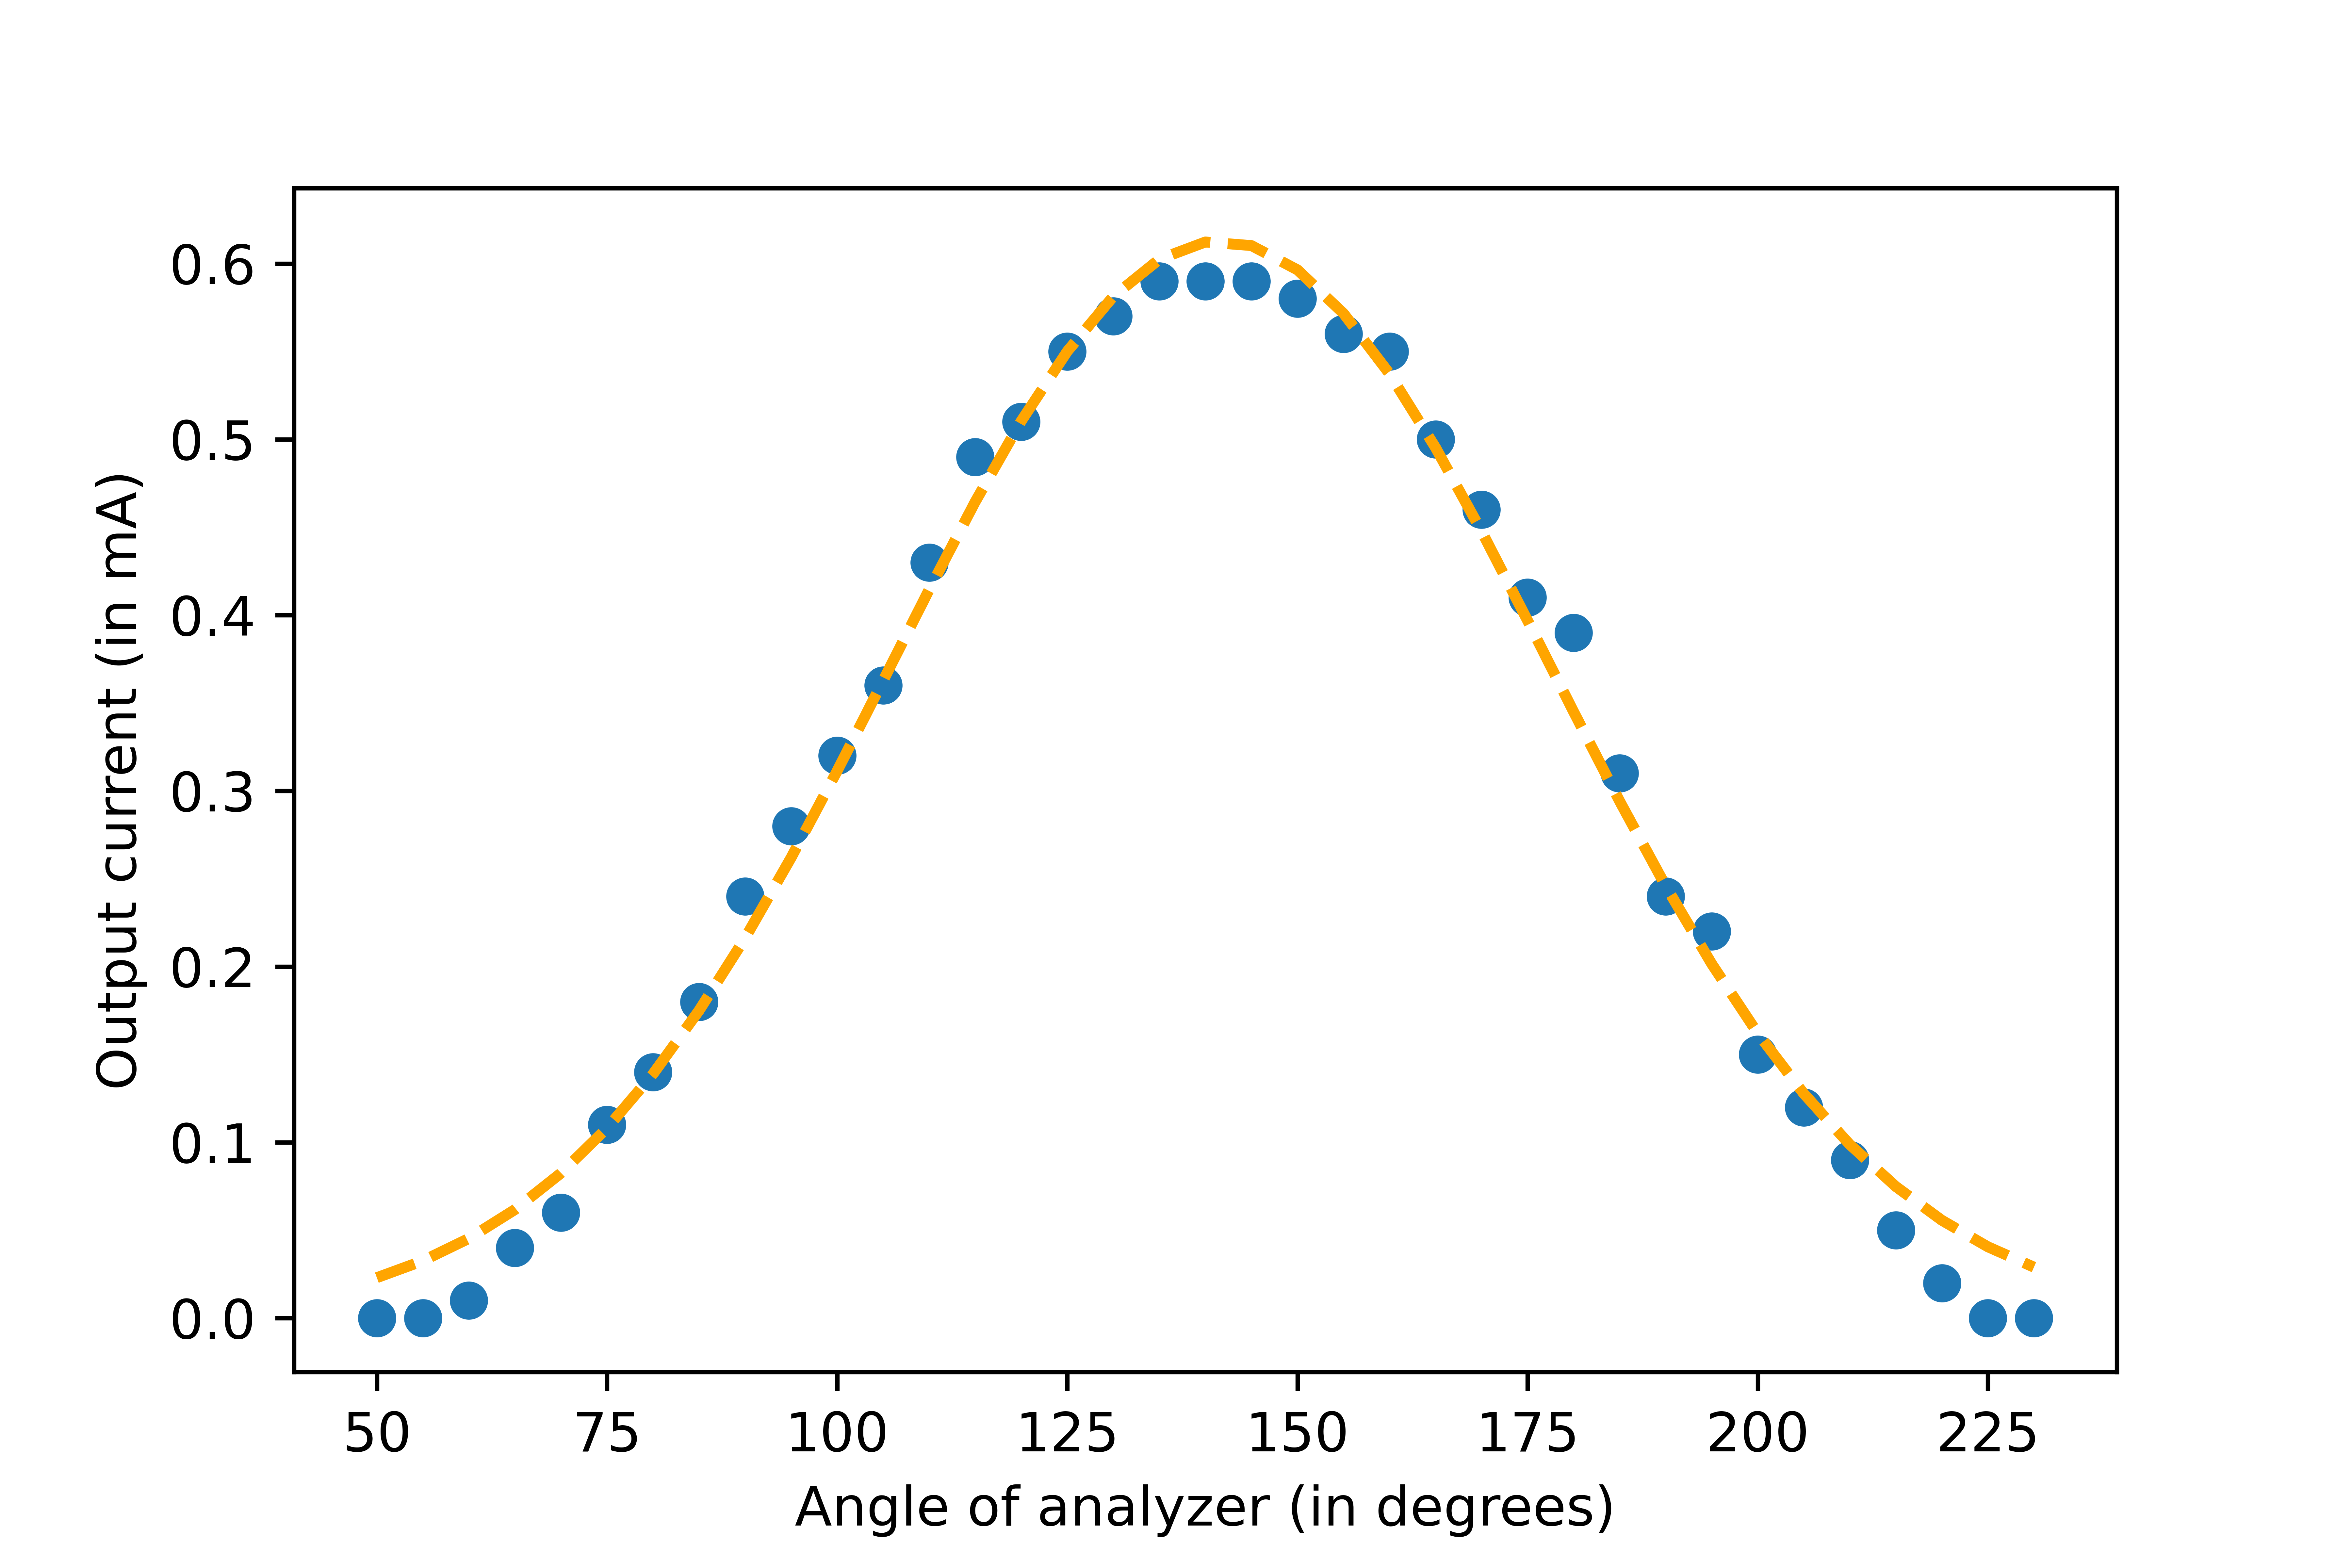
\includegraphics[scale = 0.75]{Figures/plot-1.png}
    \caption{The $I \sim \alpha$ plot for half-wave plate}
    \label{fig:my_label}
\end{figure}

\begin{figure}
    \centering
    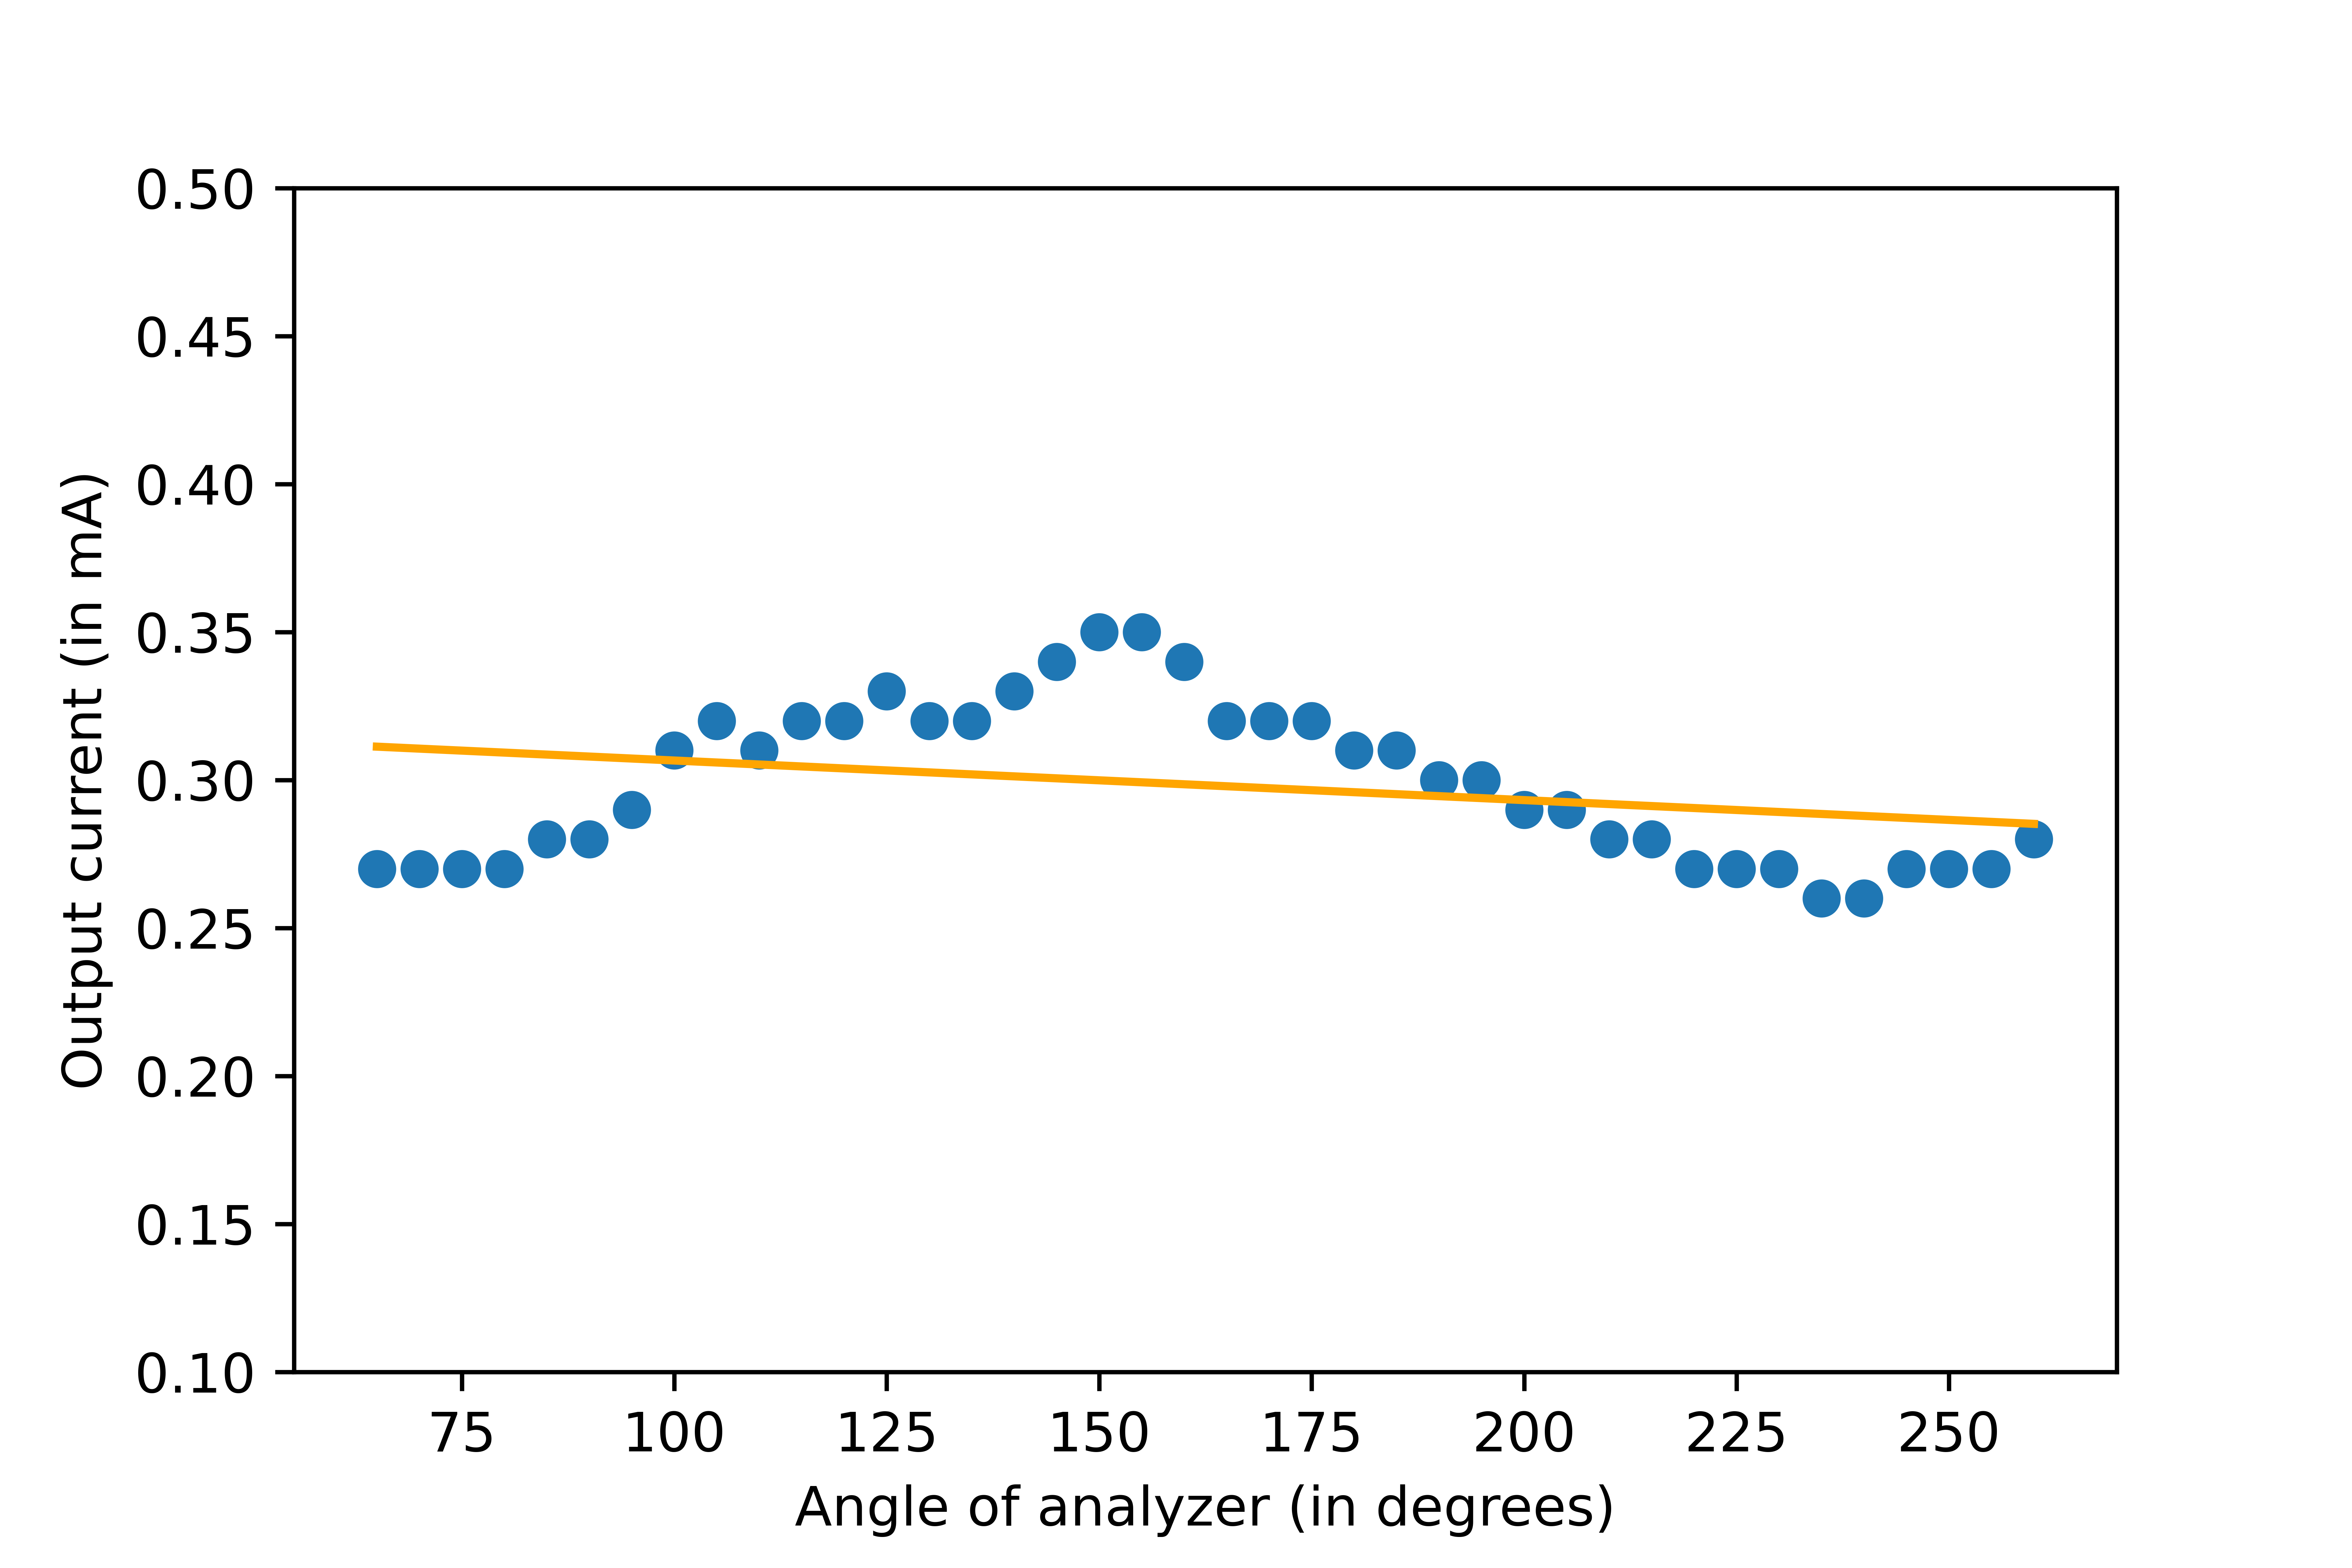
\includegraphics[scale = 0.75]{Figures/plot-2.png}
    \caption{The $I \sim \alpha$ plot for quarter-wave plate}
    \label{fig:my_label}
\end{figure}

\begin{figure}
    \centering
    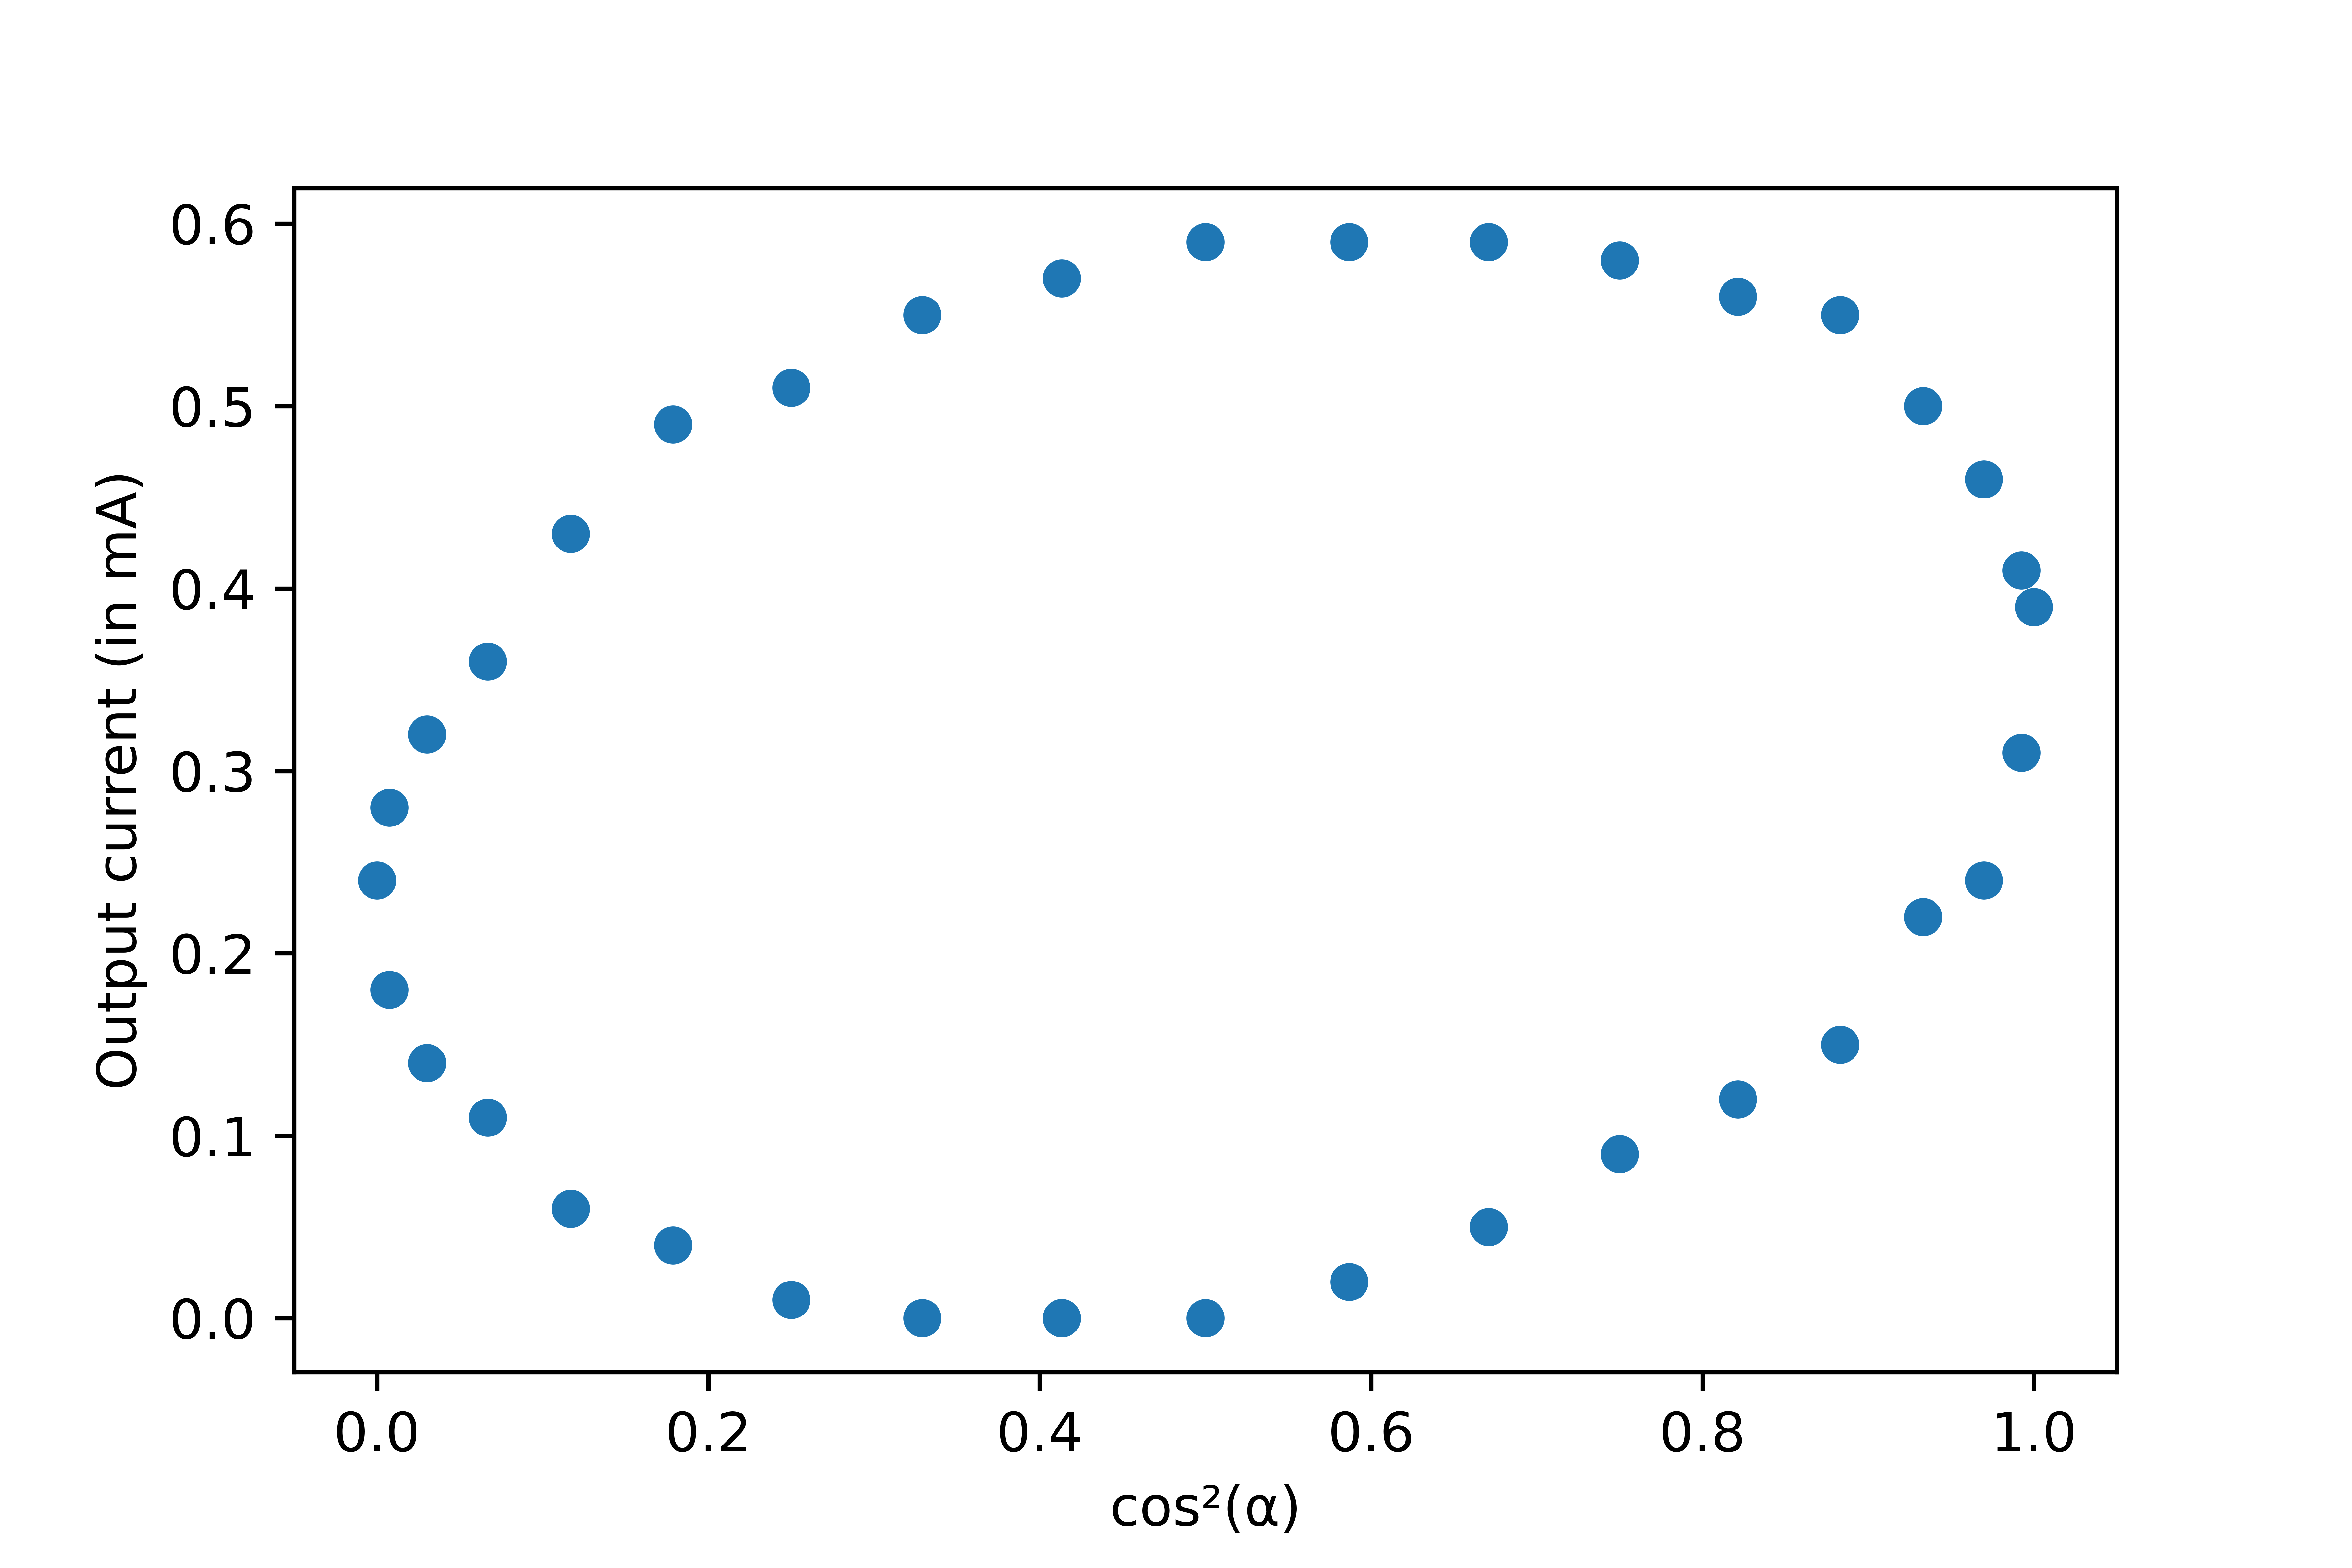
\includegraphics[scale = 0.75]{Figures/cplot-1.png}
    \caption{The $I \sim \cos^2 \alpha$ plot for half-wave plate}
    \label{fig:my_label}
\end{figure}


\begin{figure}
    \centering
    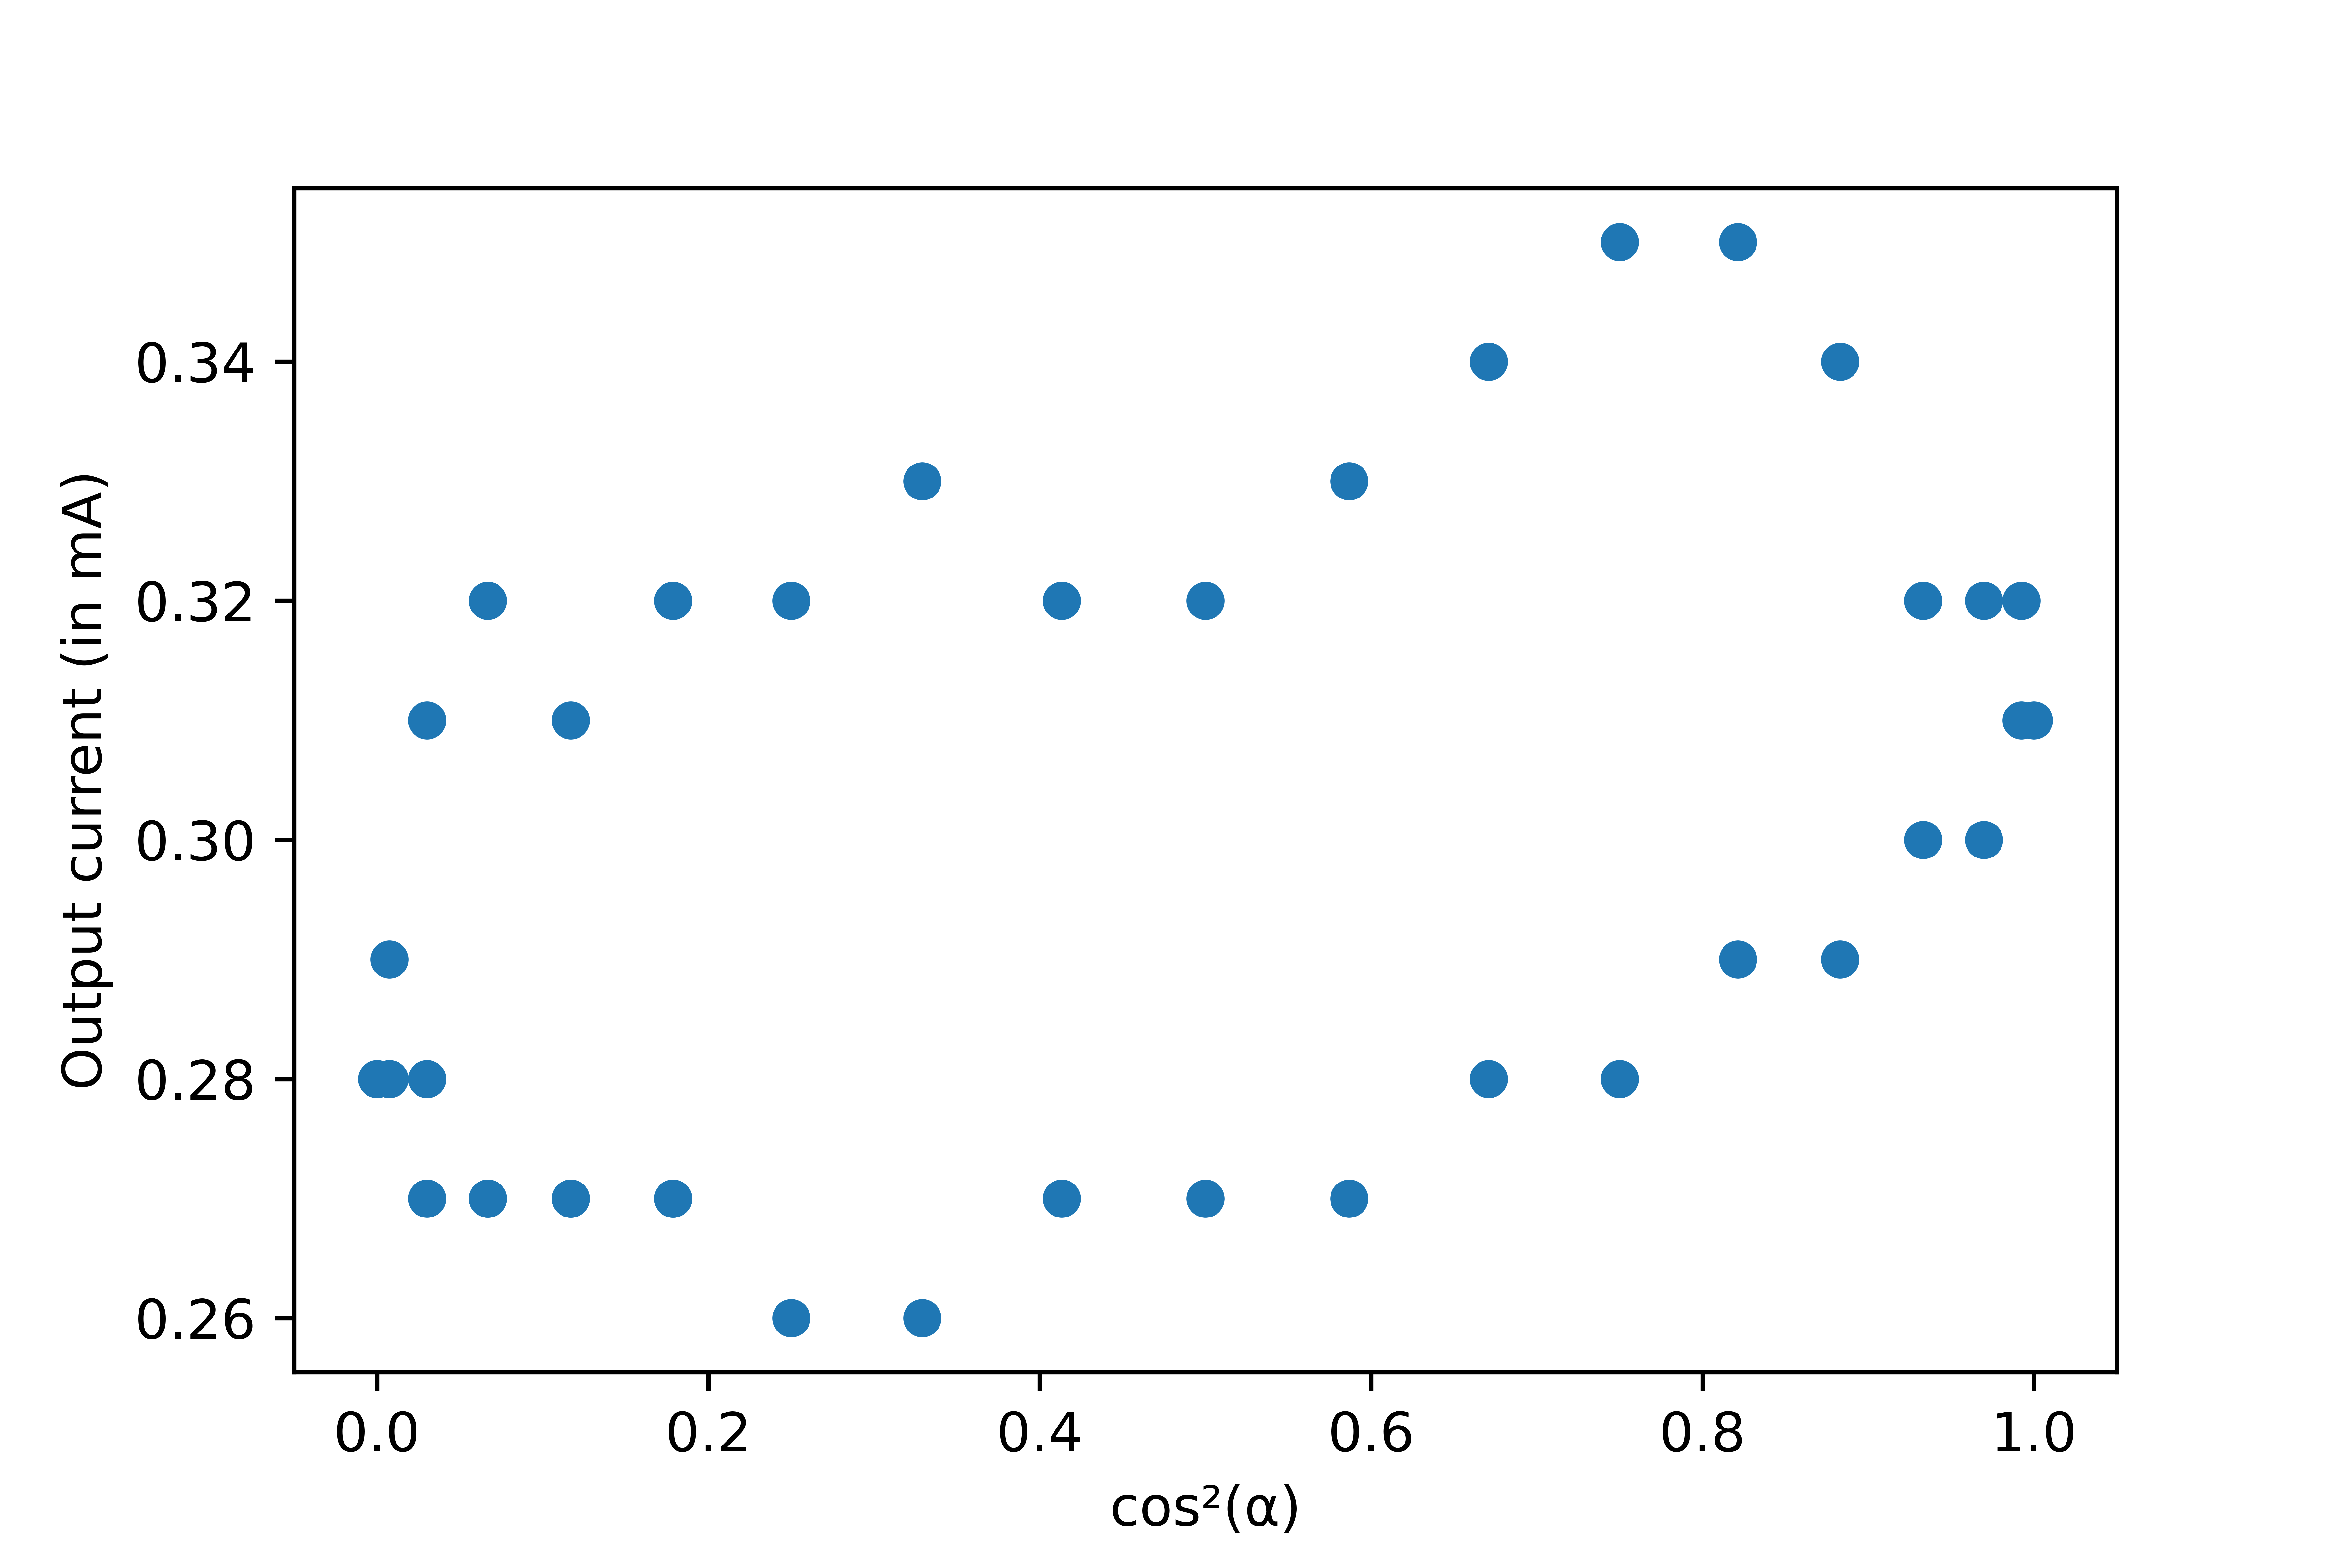
\includegraphics[scale = 0.75]{Figures/cplot-2.png}
    \caption{The $I \sim \cos^2 \alpha$ plot for quarter-wave plate}
    \label{fig:my_label}
\end{figure}



\begin{table}[!htb]
    \caption{The readings for half-wave plate}
    \begin{minipage}{.5\linewidth}
      \caption{}
      \centering
        \begin{tabular}{@{}cc@{}}
\toprule
\begin{tabular}[c]{@{}c@{}}Analyzer angle\\ (in degrees)\end{tabular} & \begin{tabular}[c]{@{}c@{}}Current\\ (mA)\end{tabular} \\ \midrule
50  & 0    \\
55  & 0    \\
60  & 0.01 \\
65  & 0.04 \\
70  & 0.06 \\
75  & 0.11 \\
80  & 0.14 \\
85  & 0.18 \\
90  & 0.24 \\
95  & 0.28 \\
100 & 0.32 \\
105 & 0.36 \\
110 & 0.43 \\
115 & 0.49 \\
120 & 0.51 \\
125 & 0.55 \\
130 & 0.57 \\
135 & 0.59 \\
140 & 0.59 \\
145 & 0.59 \\
150 & 0.58 \\
155 & 0.56 \\
160 & 0.55 \\
165 & 0.5  \\
170 & 0.46 \\
175 & 0.41 \\
180 & 0.39 \\
185 & 0.31 \\
190 & 0.24 \\
195 & 0.22 \\
200 & 0.15 \\
205 & 0.12 \\
210 & 0.09 \\
215 & 0.05 \\
220 & 0.02 \\
225 & 0    \\
230 & 0    \\ \bottomrule
\end{tabular}
    \end{minipage}%
    \begin{minipage}{.5\linewidth}
      \centering
        \caption{}
        \begin{tabular}{@{}cc@{}}
\toprule
\begin{tabular}[c]{@{}c@{}}Squared cosine of \\ analyzer angle\end{tabular} & \begin{tabular}[c]{@{}c@{}}Current\\ (mA)\end{tabular} \\ \midrule
0.41 & 0    \\
0.33 & 0    \\
0.25 & 0.01 \\
0.18 & 0.04 \\
0.12 & 0.06 \\
0.07 & 0.11 \\
0.03 & 0.14 \\
0.01 & 0.18 \\
0.00 & 0.24 \\
0.01 & 0.28 \\
0.03 & 0.32 \\
0.07 & 0.36 \\
0.12 & 0.43 \\
0.18 & 0.49 \\
0.25 & 0.51 \\
0.33 & 0.55 \\
0.41 & 0.57 \\
0.50 & 0.59 \\
0.59 & 0.59 \\
0.67 & 0.59 \\
0.75 & 0.58 \\
0.82 & 0.56 \\
0.88 & 0.55 \\
0.93 & 0.5  \\
0.97 & 0.46 \\
0.99 & 0.41 \\
1.00 & 0.39 \\
0.99 & 0.31 \\
0.97 & 0.24 \\
0.93 & 0.22 \\
0.88 & 0.15 \\
0.82 & 0.12 \\
0.75 & 0.09 \\
0.67 & 0.05 \\
0.59 & 0.02 \\
0.50 & 0    \\
0.41 & 0    \\ \bottomrule
\end{tabular}
    \end{minipage} 
\end{table}

\begin{table}[!htb]
    \caption{The readings for quarter-wave plate}
    \begin{minipage}{.5\linewidth}
      \caption{}
      \centering
        \begin{tabular}{@{}cc@{}}
\toprule
\begin{tabular}[c]{@{}c@{}}Analyzer angle\\ (in degrees)\end{tabular} & \begin{tabular}[c]{@{}c@{}}Current\\ (mA)\end{tabular} \\ \midrule
65  & 0.27 \\
70  & 0.27 \\
75  & 0.27 \\
80  & 0.27 \\
85  & 0.28 \\
90  & 0.28 \\
95  & 0.29 \\
100 & 0.31 \\
105 & 0.32 \\
110 & 0.31 \\
115 & 0.32 \\
120 & 0.32 \\
125 & 0.33 \\
130 & 0.32 \\
135 & 0.32 \\
140 & 0.33 \\
145 & 0.34 \\
150 & 0.35 \\
155 & 0.35 \\
160 & 0.34 \\
165 & 0.32 \\
170 & 0.32 \\
175 & 0.32 \\
180 & 0.31 \\
185 & 0.31 \\
190 & 0.3  \\
195 & 0.3  \\
200 & 0.29 \\
205 & 0.29 \\
210 & 0.28 \\
215 & 0.28 \\
220 & 0.27 \\
225 & 0.27 \\
230 & 0.27 \\
235 & 0.26 \\
240 & 0.26 \\
245 & 0.27 \\
250 & 0.27 \\
255 & 0.27 \\
260 & 0.28 \\ \bottomrule
\end{tabular}
    \end{minipage}%
    \begin{minipage}{.5\linewidth}
      \centering
        \caption{}
        \begin{tabular}{@{}cc@{}}
\toprule
\begin{tabular}[c]{@{}c@{}}Squared cosine of\\ analyzer angle\end{tabular} & \begin{tabular}[c]{@{}c@{}}Current\\ (mA)\end{tabular} \\ \midrule
0.18 & 0.27 \\
0.12 & 0.27 \\
0.07 & 0.27 \\
0.03 & 0.27 \\
0.01 & 0.28 \\
0.00 & 0.28 \\
0.01 & 0.29 \\
0.03 & 0.31 \\
0.07 & 0.32 \\
0.12 & 0.31 \\
0.18 & 0.32 \\
0.25 & 0.32 \\
0.33 & 0.33 \\
0.41 & 0.32 \\
0.50 & 0.32 \\
0.59 & 0.33 \\
0.67 & 0.34 \\
0.75 & 0.35 \\
0.82 & 0.35 \\
0.88 & 0.34 \\
0.93 & 0.32 \\
0.97 & 0.32 \\
0.99 & 0.32 \\
1.00 & 0.31 \\
0.99 & 0.31 \\
0.97 & 0.3  \\
0.93 & 0.3  \\
0.88 & 0.29 \\
0.82 & 0.29 \\
0.75 & 0.28 \\
0.67 & 0.28 \\
0.59 & 0.27 \\
0.50 & 0.27 \\
0.41 & 0.27 \\
0.33 & 0.26 \\
0.25 & 0.26 \\
0.18 & 0.27 \\
0.12 & 0.27 \\
0.07 & 0.27 \\
0.03 & 0.28 \\ \bottomrule
\end{tabular}
    \end{minipage} 
\end{table}




\section{Result and Discussion}

\begin{enumerate}
    \item The photo current is proportional to the light intensity.  The light intensity is proportional to the electric filed vector to the square: $I \sim E^2$.
    \item The current plot of the half-wave plate appears to a squared sinusoidal wave. This is as expected for linear polarization.
    \item The current against squared cosines of the angle is expected to be a straight. However, the plot we have is elliptical. One reason could be that the retardation was not completely by $\pi$ which could be the fault of the wave-plate. 
    \item The current of the quarter-wave plate appears to be a straight line parallel to the x-axis for the most part i.e. almost constant. We expect this for circular polarization.
    \item In circular co-ordinates we expect the plot to be a circle i.e. the radial distance acts as current (which we expect to be constant). Our plot is slightly distorted but the extremities are almost similar values. Hence, we can, for argument sake, take this to be approximated as circular behaviour. This level of distortion could be attributed to manual errors or discrepancies in the photo detector.
\end{enumerate}

\section{Conclusion}

Thus, through the experimental process we have tried to understand and visualize the two types of polarization. 



\section{Precautions}
\begin{enumerate}
    \item Do not look directly into the  light source.
    \item Make sure the polarizer, wave-plate, analyser are along the same line.
    \item Do not touch the transmitting surfaces with bare hands
    \item Turn off the source when not in use.
\end{enumerate}
\end{document}
